% ex: ts=2 sw=2 sts=2 et filetype=tex
% SPDX-License-Identifier: CC-BY-SA-4.0

\section{Comparación de algoritmos}

\begin{frame}[c]{Comparación de algoritmos}
  A menudo dispondremos de más de un algoritmo para
  resolver un problema dado, ¿con cuál nos quedamos?

  \pausa
  \vspace{\baselineskip}
  \textbf{Uso de recursos}

  \vspace{\baselineskip}
  \begin{itemize}
    \item Computacionales:
          \begin{itemize}
            \item Tiempo de ejecución
            \item Espacio de memoria
          \end{itemize}
    \item No computacionales:
          \begin{itemize}
            \item Esfuerzo de desarrollo (análisis, diseño e implementación)
          \end{itemize}
  \end{itemize}
\end{frame}

\begin{frame}[c]{Factores que influyen en el uso de recursos}
  \begin{itemize}
    \item Recursos computaciones:
          \begin{itemize}
            \item Diseño del algoritmo
            \pausa
            \item Complejidad del problema (p.ej. tamaño de las entradas)
            \pausa
            \item Hardware (arquitectura, MHz, MBs...)
            \pausa
            \item Calidad del código
            \pausa
            \item Calidad del compilador (optimizaciones)
          \end{itemize}
    \pausa
    \item Recursos no computaciones:
          \begin{itemize}
            \item Complejidad del algoritmo
            \pausa
            \item Disponibilidad de biblioteca reutilizables
          \end{itemize}
  \end{itemize}
\end{frame}

\section{Principio de invarianza}

\begin{frame}[c]{Principio de invarianza}
  \begin{itemize}
    \item Dos implementaciones de un mismo algoritmo no deferirán más
      que en una constante multiplicativa.
    \pausa
    \item Si $t_1(n)$ y $t_2(n)$ son los tiempos de dos implementaciones
      de un mismo algoritmo, se pude comprobar que:

      \vspace{\baselineskip}
      $\exists c,d \in \mathbb{R}, t_1(n) \leq ct_2()n); t_2(n) \leq dt_1(n)$
  \end{itemize}
\end{frame}

\section{Eficiencia}

\begin{frame}[c]{Eficiencia}
  Medida del uso de los recursos computacionales
  requeridos por la ejecución de un algoritmo en función
  del tamaño de las entradas.

  \vspace{\baselineskip}
  \begin{description}
    \item[T(n)] Tiempo empleado para ejecutar el algoritmo con una entrada
      de tamaño \textbf{n}
  \end{description}
\end{frame}

\begin{frame}[c]{Tipos de análisis}
  ¿Cómo medios el tiempo de ejecución de un algoritmo?

  \vspace{\baselineskip}
  \begin{description}
    \item[Mejor caso] En condiciones óptimas (no se usa por ser
      demasiado optimista).
    \pausa
    \item[Peor caso] En el peor escenario posible (nos permite acotar
      el tiempo de ejecución).
    \pausa
    \item[Caso promedio] Caso difícil de caracterizar en la práctica.
    \pausa
    \item[Análisis probabilístico] Asume una distribución de probabilidad
      sobre las posibles entradas.
    \pausa
    \item[Análisis amortizado] Tiempo medio de ejecución por operación
      sobre una secuencia de ejecuciones sucesivas.
  \end{description}
\end{frame}

\begin{frame}[c]{Ejemplo}

  \begin{table}[]
  \begin{tabular}{ll}
    Algoritmo 1:  & $T(n) = 10^{-4} 2^{n}$ segundos\\
    & $n = 38$ datos\\
    & $T(n) = $ 1 año\\
  \end{tabular}
  \end{table}
  \begin{table}[]
  \begin{tabular}{ll}
    Algoritmo 2:  & $T(n) = 10^{-2} n^{3}$ segundos\\
    & $n = 1000$ bits\\
    & $T(n) = $ 1 año\\
  \end{tabular}
  \end{table}

  \vspace{\baselineskip}
  ¿Cuál es mejor? Se precisa un \textbf{análisis asintótico}
\end{frame}

\section{Notaciones asintóticas}

\begin{frame}[c]{Notaciones asintóticas}
  Estudian el comportamiento del algoritmo cuando el
  tamaño de las entradas es lo suficientemente grande,
  sin tener en cuenta lo que ocurre para entradas
  pequeñas y obviando factores constantes.
\end{frame}

\begin{frame}[c]{Orden de eficiencia}
  Un algoritmo tiene un tiempo de ejecución de \textbf{orden
  f(n)}, para una función dada $f$, si existe una constante
  positiva $c$ y una implementación del algoritmo capaz
  de resolver cada caso del problema en un \textbf{tiempo 
  acotado superiormente por $c f(n)$}, donde $n$ es el
  tamaño del problema considerado.
\end{frame}

\begin{frame}[c]{Notación O}
  Decimos que una función \textbf{T(n)} es \textbf{O(f(n))}
  si existen constantes $n_0$ y $c$ tales que $T(n) \leq cf(n)$
  para todo $n \geq n_0$:

  \vspace{\baselineskip}
  \begin{math}
    T(n) \textrm{ es } O(f(n)) \iff \exists c \in \mathbb{R}, \exists n_0 \in \mathbb{N},
    | \forall n > n_0 \in \mathbb{N}, T(n) \leq cf(n)
  \end{math}

  \vspace{\baselineskip}
  \begin{center}
    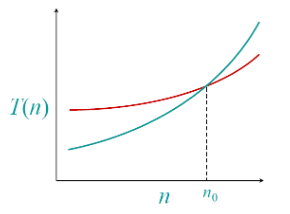
\includegraphics[scale=0.4]{03-tn_n_n0.png}
  \end{center}
\end{frame}

\begin{frame}[c]{Ejemplos}
  T(n) = 3n
  \begin{itemize}
    \item T(n) es O(n), O(n log n), O($n^2$), O($n^3$) y O($2^n$).
  \end{itemize}

  \pausa
  T(n) = $(n+1)^2$
  \begin{itemize}
    \item O($n^2$), O($n^3$) y O($2^n$).
    \item T(n) no es O(n) ni O(n log n).
  \end{itemize}

  \pausa
  T(n) = $32n^2 + 17n + 32$
  \begin{itemize}
    \item T(n) es O($n^2$) pero no es O(n).
  \end{itemize}

  \pausa
  T(n) = $3n^3 + 345n^2$
  \begin{itemize}
    \item T(n) es O($n^3$) pero no es O($n^2$).
  \end{itemize}

  \pausa
  T(n) = $3^n$
  \begin{itemize}
    \item T(n) es O($3^n$) pero no es O($n^2$).
  \end{itemize}
\end{frame}

\begin{frame}[c]{Notaciones $\Omega$ y $\Theta$}
  \begin{block}{Notación $\Omega$ (cota inferior)}
    T(n) es $\Omega$(f(n)) cuando

    \begin{math}
      \exists c \in \mathbb{R}^+, \exists n_0 \in \mathbb{N}:
      \forall n \geq n_0 \implies T(n) \geq cf(n)
    \end{math}
  \end{block}

  \pausa
  \begin{block}{Notación $\Theta$ (orden exacto)}
    T(n) es $\Theta$(f(n)) cuando

    T(n) es O(f(n)) y T(n) es $\Theta$(f(n))
  \end{block}
\end{frame}

\section{Cálculo de la eficiencia de un algoritmo}

\begin{frame}[c]{Órdenes de eficiencia más habituales}
  \begin{center}
    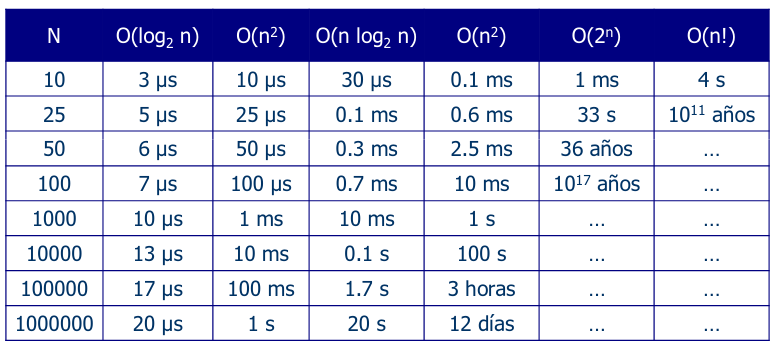
\includegraphics[scale=0.4]{03-tabla_eficiencia.png}
  \end{center}
  Tiempos calculados suponiendo $1 \mu{}s$ por operación elemental.

  \begin{math}
    O(1) \subset O(log n) \subset O(n) \subset O(n log n) \subset
    O(n^2) \subset O(n^3) \subset O(2^n) \subset O(n!)
  \end{math}
\end{frame}

\begin{frame}[fragile]
  \frametitle{Órdenes de eficiencia}

  \begin{lstlisting}[language=C]
  max = a[0]
  for i = 2 to n {
    if (a[i] > max)
      max = a[i]
  }
  \end{lstlisting}
\end{frame}

\section{Resolución de recurrencias}

\begin{frame}[c]{}
\end{frame}

